\subsection{Cantidad de paquetes por cada campo Type}

A continuación, se mostrará una breve descripción de cada uno de los tipos de los paquetes ethernet.

\underline{Protocolo ARP (Address Resolution Protocol):}

Es el protocolo encargado de encontrar la dirección MAC que corresponde a una determinada dirección IP. Para lograrlo, se envía un request ARP a la dirección de la red con MAC = FF FF FF FF FF FF, que contiene la dirección IP por la que se está preguntando. Se espera que esa máquina responda un reply ARP con la dirección IP que le corresponde.

\underline{Protocolo IP (Internet Protocol):}

Su función principal es el uso bidireccional en origen o destino de comunicación para transmitir datos mediante un protocolo no orientado a conexión que transfiere paquetes a través de distintas redes físicas.
En este protocolo no se necesita ninguna configuración antes de que un equipo intente enviar paquetes a otro con el que no se había comunicado antes.

\underline{Protocolos IPv4 (Internet Protocol version 4) y IPv6 (Internet Protocol version 6):}

IPv4 es la cuarta versión del protocolo IP, y actualmente es usada en la gran mayoría de dispositivos que acceden a Internet. IPv6 se diseñó para reemplazar a IPv4 ya que admite una mayor cantidad de direcciones de host diferentes.

\underline{Protocolo LLDP (Link Layer Discovery Protocol):}

Es utilizado por los dispositivos de la red para hacer públicos su identidad, capacidades y vecinos en una LAN IEEE 802, principalmente por cable Ethernet.
El LLDP puede ser utilizado como componente en aplicaciones de gestión de red y monitoreo.
	
\underline{LLC (Logical Link Control):}

Es la subcapa de enlace de datos responsable del control de enlace lógico. Además, maneja el control de errores, control del flujo, control de diálogo y direccionamiento de la subcapa MAC.
Los protocolos LLC son utilizados para la comunicación entre entidades de la propia subcapa LLC. También definen los procedimientos para el intercambio de tramas de información y de control entre cualquier par de puntos. 
El protocolo LLC más generalizado es IEEE 802.2.



Para cada red estudiada se presenta un gráfico con el porcentaje de paquetes tranmitidos para cada protocolo y su análisis del overhead impuesto por ARP.

\subsubsection{Red Hogareña}

\centerline{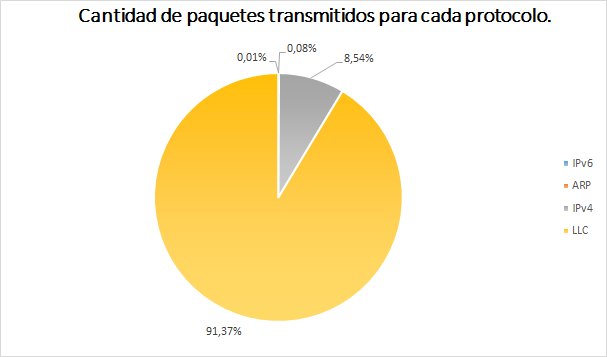
\includegraphics[width=0.8\textwidth]{./graficos/paquetesVSProtocolo/casa_mari2.png}}

Como se puede observar, la cantidad de paquetes arp es muy baja con respecto a los otros protocolos. Suponemos que se debe a que no se conectaron nuevos dispositivos y la mayoría de éstos ya eran conocidos por la red. A partir de este gráfico, se puede notar que el overhead impuesto por ARP es muy bajo.

\subsubsection{Red Laboratorio}

\centerline{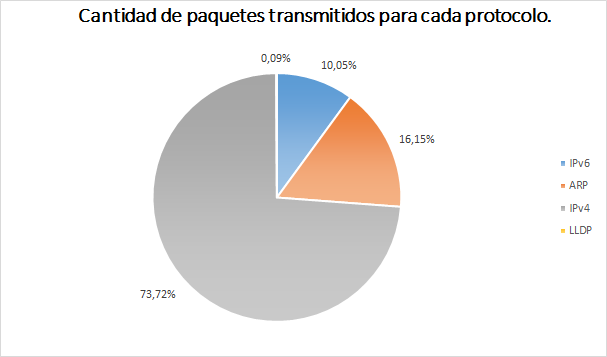
\includegraphics[width=0.8\textwidth]{./graficos/paquetesVSProtocolo/labo52.png}}
	
La sobrecarga de paquetes ARP presentada en esta red es mucho mayor a la anterior debido a que la red es mucho más grande que la anterior.

\subsubsection{Red Devartis}

\centerline{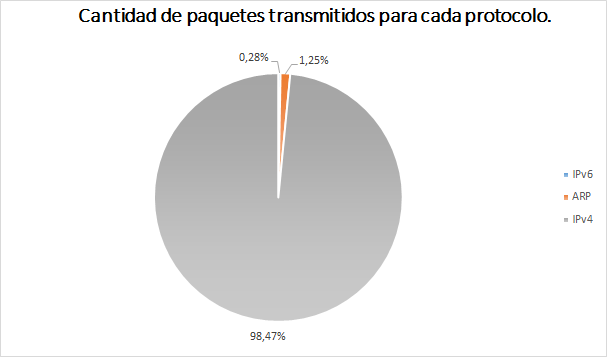
\includegraphics[width=0.8\textwidth]{./graficos/paquetesVSProtocolo/laburo_mari2.png}}

\subsubsection{Red Mercap}

\centerline{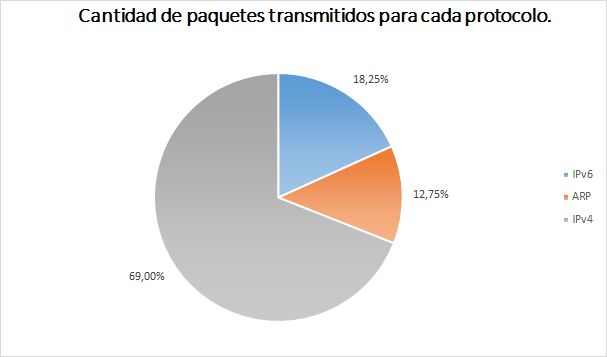
\includegraphics[width=0.8\textwidth]{./graficos/paquetesVSProtocolo/laburo_eze2.png}}


Analizando los gráficos obtenidos a partir de cada red, se puede notar que el porcentaje de paquetes ARP con respecto al resto de los protocolos es bajo. Comparándolos entre sí, se puede apreciar que cuanto más grande es la red mayor es el overhead impuesto por ARP.

Podemos agregar que el overhead afeta al throughput (cantidad de datos que se entregan por unidad de tiempo) de una conexión. Esto se debe que hay un "desperdicio" de ancho de banda, causado por la información adicional (control, secuencia, etc) que debe viajar en los paquetes además de los datos, ya que estos datos extra no contribuyen al contenido del mensaje.